\chapter{Intermediate Memory Topics}
\label{memoryintermediate}

\section{How a Computer Views Memory}

Let's review how memory within a computer works.  You may also want to
re-read \autoref{computerarchitecture}.

A computer looks at memory as a long sequence of numbered storage
locations.  A sequence of \emph{millions} of numbered
storage locations.  Everything is stored in these locations.  Your
programs are stored there, your data is stored there, everything.  
Each storage location looks like every other one.  The locations 
holding your program are just like the ones holding your data.  In
fact, the computer has no idea which are which, except that the
executable file tells it where to start executing.

These storage locations are called bytes.  The computer can combine
up to four of them together into a single word.  Normally numeric
data is operated on a word at a time.  As we mentioned, instructions
are also stored in this same memory.  Each instruction is a different
length.  Most instructions take up one or two storage locations for
the instruction itself, and then storage locations for the instruction's
arguments.  For example, the instruction

\begin{simpletyping}
\begin{lstlisting}
	movl data\_items(,{\ediBare},4), {\ebxBare}
\end{lstlisting}
\end{simpletyping}

takes up 7 storage locations.  The first two hold the instruction,
the third one tells which registers to use, and the next four hold
the storage location of \icode{data\_items}.  In memory,
instructions look just like all the other numbers, and the instructions themselves
can be moved into and out of registers just like numbers, because that's
what they are.

This chapter is focused on the details of computer memory.  To get started
let's review some basic terms that we will be using in this chapter:

\begin{description}
\item[Byte] This is the size of a storage location.  On x86 processors, a byte
can hold numbers between 0 and 255.
\item[Word] This is the size of a normal register.  On x86 processors, a word
is four bytes long.  Most computer operations handle a word at a time.
\item[Address] An address is a number that refers to a byte in memory.  For example, the first
byte on a computer has an address of 0, the second has
an address of 1, and so on.\footnote{You actually never use
addresses this low, but it works for discussion.}
Every piece of data on the computer not in a register has an address.
The address of data which spans several bytes is the same as the address
of its first byte.

Normally, we don't ever type the numeric address of anything, but we let the
assembler do it for us.  When we use labels in code, the
symbol used in the label will be equivalent to the address it is labelling.  The assembler
will then replace that symbol with its address wherever you use it in 
your program.  For example, say you have the following code:

\begin{simpletyping}
\begin{lstlisting}
	.section .data
my\_data:
	.long 2, 3, 4
\end{lstlisting}
\end{simpletyping}

Now, any time in the program that \icode{my\_data} is used, 
it will be replaced by the address of the first value of the \icode{.long}
directive.
\item[Pointer] A pointer is a register or memory word whose value is an 
address.  In our programs we use \icode{{\ebpBare}} as a pointer
to the current stack frame.  All base pointer addressing involves pointers.
Programming uses a lot of pointers, so
it's an important concept to grasp.
\end{description}

\section{The Memory Layout of a Linux Program}

When you program is loaded into memory, each \icode{.section\index{.section}}
is loaded into its own region of memory.  All of the code and data declared
in each section is brought together, even if they were separated in your
source code.

The actual instructions (the \icode{.text\index{.text}} section) are loaded at the 
address 0x08048000 (numbers starting with \icode{0x} are in hexadecimal, which
will be discussed in \autoref{countingchapter}).\footnote{Addresses mentioned in this chapter are not set in stone and may vary based on kernel 
version.}  The \icode{.data\index{.data}}
section is loaded immediately after that, followed by the 
\icode{.bss\index{.bss}}
section.

The last byte that can be addressed on Linux is location
0xbfffffff.  Linux starts the stack here and grows
it downward toward the other sections.  Between them is a huge 
gap.  The initial layout of the stack is as follows:
At the bottom of the stack (the bottom of the stack is the
top address of memory - see \autoref{functionschapter}),
there is a word of memory that is
zero.  After that comes the null-terminated 
name of the program using ASCII characters.
After the program name comes the program's environment variables (these
are not important to us in this book).  Then come the program's command-line arguments.
These are the values that the user typed in on the command line
to run this program.  When we run \icode{as},
for example, we give it several arguments - \icode{as},
\icode{sourcefile.s}, \icode{-o}, and 
\icode{objectfile.o}.  After these, we have the 
number of arguments that were used.  When the program begins,
this is where the stack pointer, {\espRegIdx}, is pointing.  
Further pushes on the stack move {\espReg} down in memory.  For example,
the instruction

\begin{simpletyping}
\begin{lstlisting}
	pushl {\eaxBare}
\end{lstlisting}
\end{simpletyping}

is equivalent to

\begin{simpletyping}
\begin{lstlisting}
	movl {\eaxBare}, ({\espBare})
	subl \$4, {\espBare}
\end{lstlisting}
\end{simpletyping}

Likewise, the instruction

\begin{simpletyping}
\begin{lstlisting}
	popl {\eaxBare}
\end{lstlisting}
\end{simpletyping}

is the same as

\begin{simpletyping}
\begin{lstlisting}
	movl ({\espBare}), {\eaxBare}
	addl \$4, {\espBare}
\end{lstlisting}
\end{simpletyping}

Your program's data region starts at the bottom of memory and goes up.
The stack starts at the top of memory, and moves downward with each push.
This middle part between the stack and your program's data sections is 
inaccessible memory - you are not allowed to 
access it until you tell the kernel that you need it.\footnote{The
stack can access it as it grows downward, and you can access the stack
regions through {\espRegIdx}.  However, your program's data section
doesn't grow that way.  The way to grow that will be explained shortly.}
If you try, you
will get an error (the error message is usually "segmentation fault").  
The same will happen if you try to
access data before the beginning of your program, 0x08048000.  
The last accessible memory address to your program is called the 
\emph{system break\index{system break}}
(also called the \emph{current break\index{current break}} or just the \emph{break}).

\begin{figure}
\caption{Memory Layout of a Linux Program at Startup}
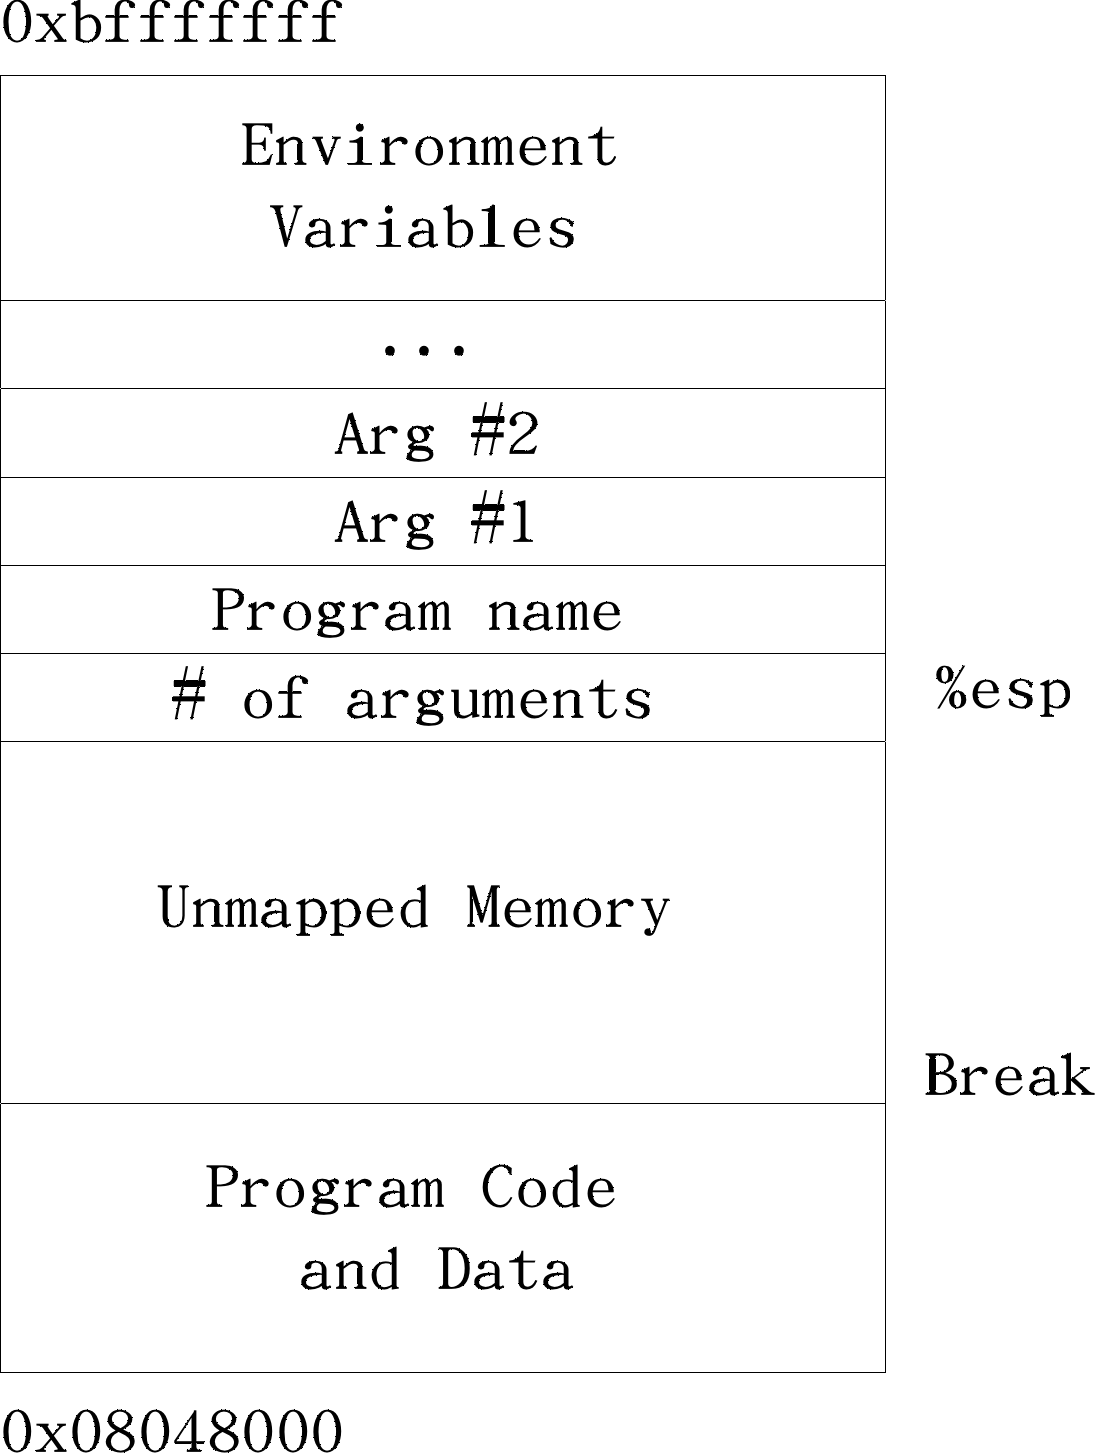
\includegraphics[width=\textwidth]{memorylayout.png}
\end{figure}

\section{Every Memory Address is a Lie}

So, why does the computer not allow you to access memory in the 
break area?  To answer this question, we will have to delve into
the depths of how your computer really handles memory.  

You may have wondered, since every program gets loaded into the same
place in memory, don't they step on each other, or overwrite each other?
It would seem so.  However, as a program writer, you only access
\emph{virtual memory\index{virtual memory}}.  

\emph{Physical memory\index{physical memory}}
refers to the actual RAM chips inside your computer and what they contain.   It's usually
between 16 and 512 Megabytes on modern computers.  If we talk about a \emph{physical
memory address}, we are talking about where exactly on these
chips a piece of memory is located.  Virtual
memory is the way \emph{your program} thinks about memory.  Before loading
your program, Linux finds an empty physical memory space large enough to
fit your program, and then tells
the processor to pretend that this memory is actually at the address
0x0804800 to load your program into.  Confused yet?  Let me explain further.

Each program gets its own sandbox to play in.  Every program running
on your computer thinks that it was loaded at memory address 0x0804800,
and that its stack starts at 0xbffffff.  When Linux loads a program,
it finds a section of unused memory, and then tells the processor to use
that section of memory as the address 0x0804800 for this program.  The
address that a program believes it uses is called the 
virtual address\index{virtual address},
while the actual address on the chips that it refers to is called
the physical address\index{physical address}.  
The process of assigning virtual addresses to
physical addresses is called 
\emph{mapping\index{mapping}}.  

Earlier we 
talked about the inaccessible memory between the \icode{.bss} and the 
stack, but we didn't talk about why it was there.  The reason is that this
region of virtual memory addresses hasn't been mapped onto 
physical memory addresses.  The mapping process takes up considerable
time and space, so if every possible virtual address of every possible
program were mapped, you would not have enough physical memory to even run one program.  So,
the break is the beginning of the area that contains unmapped memory.  With the
stack, however, Linux will automatically map in memory that is accessed from
stack pushes.

Of course, this is a very simplified view of virtual memory.  The full 
concept is much more advanced.  For example, 
Virtual memory can be mapped to more than just physical memory; it
can be mapped to disk as well.  Swap partitions on Linux allow
Linux's virtual memory system to map memory not only to physical RAM,
but also to disk blocks as well.  For example, let's
say you only have 16 Megabytes of physical memory.  Let's also say that
8 Megabytes are being used by Linux and some basic applications, and you
want to run a program that requires 20 Megabytes of memory.  Can you?  The
answer is yes, but only if you have set up a swap partition.  What
happens is that after all of your remaining 8 Megabytes of physical memory
have been mapped into virtual memory, Linux starts mapping parts of your application's
virtual memory to disk blocks.  So, if you access a "memory" location in your
program, that location may not actually be in memory at all, but on
disk.  As the programmer you won't know the difference, though, because 
it is all handled behind the scenes by Linux.

Now, x86 processors cannot run instructions directly from disk, nor can
they access data directly from disk.  This requires the help of the operating
system.  When you try to access memory that is mapped to disk, the processor
notices that it can't service your memory request directly.  It then asks
Linux to step in.  Linux notices that the memory
is actually on disk.  Therefore, it moves some data that is currently in 
memory onto disk to make room, and then moves the memory being accessed
from the disk back into physical memory.  It then adjusts the processor's
virtual-to-physical memory lookup tables so that it can find the memory in
the new location.  Finally, Linux returns control to the program and restarts
it at the instruction which was trying to access the data in the first place.  
This instruction can now be completed successfully, 
because the memory is now in physical RAM.\footnote{Note that not only 
can Linux have a virtual address map to a different
physical address, it can also move those mappings around as needed.
}

Here is an overview of the way memory accesses are handled under Linux:

\begin{itemize}\item The program tries to load memory from a virtual address. 
\item The processor, using tables supplied by Linux, transforms the virtual memory address into a physical memory address on the fly. 
\item If the processor does not have a physical address listed for the memory address, it sends a request to Linux to load it. 
\item Linux looks at the address.  If it is mapped to a disk location, it continues on to the next step.  Otherwise, it terminates the program with a segmentation fault error. 
\item If there is not enough room to load the memory from disk, Linux will move another part of the program or another program onto disk to make room. 
\item Linux then moves the data into a free physical memory address. 
\item Linux updates the processor's virtual-to-physical memory mapping tables to reflect the changes. 
\item Linux restores control to the program, causing it to re-issue the instruction which caused this process to happen. 
\item The processor can now handle the instruction using the newly-loaded memory and translation tables. 
\end{itemize}

It's a lot of work for the operating system, but it gives the user and the programmer great
flexibility when it comes to memory management.

Now, in order to make the process more efficient,
memory is separated out into groups called \emph{pages\index{pages}}.  When
running Linux on x86 processors, a page is 4096 bytes of memory.
All of the memory mappings are done a page at a time.  Physical memory assignment,
swapping\index{swapping}, mapping, etc. are all done to memory pages\index{memory pages} instead of individual memory
addresses.  What this means to you as a programmer
is that whenever you are programming, you should try to keep most memory accesses within
the same basic range of memory, so you will only need a page or two of memory at
a time.  Otherwise, Linux may have to keep moving pages on and off of disk to 
satisfy your memory needs. Disk access is slow, so this can really slow down your program. 

Sometimes so many programs can be loaded that there is hardly enough physical
memory for them.  They wind up spending more time just swapping memory on and off of disk
than they do actually processing it.  This leads to a condition called 
\emph{swap death\index{swap death}}
which leads to your system being unresponsive and unproductive.  It's usually
usually recoverable if you start terminating your memory-hungry programs, but it's a pain.

\begin{sidebar}[Resident Set Size]
The amount of memory that your program currently has in physical memory is called its
resident set size\index{resident set size}, and
can be viewed by using the program \icode{top}.  The resident set size
is listed under the column labelled "RSS".
\end{sidebar}

\section{Getting More Memory}
\label{dynamicmemory}

We now know that Linux maps all of our virtual memory into physical memory or
swap.  If you try to access a piece of virtual memory\index{virtual memory} 
that hasn't been mapped yet,
it triggers an error known as a segmentation fault, which will terminate your 
program.  The program break point, if you remember, is the last valid address you
can use.  Now, this is all great if you know beforehand how much storage you will
need.  You can just add all the memory you need to your \icode{.data}
or \icode{.bss} sections, and it will
all be there.  However, let's say you don't know how much memory you will need.  For example,
with a text editor, you don't know how long the person's file will be.  You could try
to find a maximum file size, and just tell the user that they can't go beyond that, but
that's a waste if the file is small.  Therefore Linux has a facility to move the break point
to accomodate an application's memory needs.

If you need more memory, you can just tell Linux where you want the new break point
to be, and Linux will map all the memory you need between the current and new break
point, and then move the break point to the spot you specify.  That memory is now
available for your program to use.  The
way we tell Linux to move the break point is through the 
\icode{brk\index{brk}} 
system call.  The \icode{brk} system call is call number
45 (which will be in {\eaxReg}).  {\ebxReg} should be loaded with the requested breakpoint.  
Then you call \icode{int \$0x80} to signal Linux to do its work.  
After mapping in your memory, Linux will return the new break point in {\eaxReg}.
The new break point might actually be larger
than what you asked for, because Linux rounds up to the nearest page.  If there is
not enough physical memory or swap to fulfill your request, Linux will return a zero
in {\eaxReg}.  Also, if you call \icode{brk} with a zero in {\ebxReg}, it will
simply return the last usable memory address.

 

The problem with this method is keeping track of the memory we request.  Let's say I need to
move the break to have room to load a file, and then need to move a break again to
load another file.  Let's say I then get rid of the first file.  You now have
a giant gap in memory that's mapped, but that you aren't using.  If you continue to 
move the break in this way for each file you load, you can easily run out of memory.  
So, what is needed is a \emph{memory manager\index{memory manager}}.  

A memory manager is a set of routines that takes care of the dirty work of getting
your program memory for you.  Most memory managers have two basic functions - 
\icode{allocate} and \icode{deallocate}.\footnote{The function 
names usually aren't \icode{allocate} and \icode{deallocate}, but
the functionality will be the same.  In the C programming language, for example, they
are named \icode{malloc} and \icode{free}.}
Whenever you need a certain amount of memory, you can simply tell \icode{allocate}
how much you need, and it will give you back an address to the memory.  
When you're done with it, you tell \icode{deallocate}
that you are through with it.  \icode{allocate} will then be able to reuse the
memory.  This pattern of memory management is called \emph{dynamic memory allocation\index{dynamic memory allocation}}.  
This minimizes the number of "holes" in your memory, making sure that you
are making the best use of it you can.
The pool of memory used by memory managers
is commonly referred to as 
\emph{the heap\index{heap}}.

The way memory managers work is that they keep track of where the system break is, and
where the memory that you have allocated is.  
They mark each block of memory in the heap as
being used or unused.  When you request memory, the memory manager checks to see if there
are any unused blocks of the appropriate size.  If not, it calls the \icode{brk}
system call to request more memory.  When you free memory it marks the block as unused
so that future requests can retrieve it.  In the next section we will look at building
our own memory manager.

\section{A Simple Memory Manager}

Here I will show you a simple memory manager.  It is very primitive but it shows the 
principles quite well.
As usual, I will give you the program first for you to look through.  Afterwards will follow
an in-depth explanation.  It looks long, but it is mostly comments.

\begin{simpletyping}
\lstinputlisting{alloc.s}
\end{simpletyping}

The first thing to notice is that there is no \icode{\_start} symbol.  The reason
is that this is just a set of functions.  A memory manager by itself is not a full 
program - it doesn't do anything.  It is simply a utility to be used by other programs.

To assemble the program, do the following:

\begin{simpletyping}
\begin{lstlisting}
as alloc.s -o alloc.o
\end{lstlisting}
\end{simpletyping}

Okay, now let's look at the code.

\section{Variables and Constants}

At the beginning of the program, we have two locations set up:

\begin{simpletyping}
\begin{lstlisting}
heap\_begin:
	.long 0

current\_break:
	.long 0
\end{lstlisting}
\end{simpletyping}

Remember, the section of memory being managed is commonly referred to as
the \emph{heap\index{heap}}. 
When we assemble the program, we have no idea where the beginning of the heap is, nor 
where the current break\index{current break} 
is.  Therefore, we reserve space for their addresses, but just fill them with a 0 for the
time being.  

Next we have a set of constants to define the structure of the heap.  The way this
memory manager works is that before each region of memory allocated, we will have a 
short record describing the memory.
This record has a word reserved for the available flag and a word for the region's size.
The actual memory allocated immediately follows this record.  The available flag is used
to mark whether this region is available for allocations, or if it is currently in
use.  The size field lets us know both whether or not this region is big enough for
an allocation request, as well as the location of the next memory region.
The following constants describe this record:

\begin{simpletyping}
\begin{lstlisting}
	.equ HEADER\_SIZE, 8
	.equ HDR\_AVAIL\_OFFSET, 0
	.equ HDR\_SIZE\_OFFSET, 4
\end{lstlisting}
\end{simpletyping}

This says that the header is 8 bytes total, the available flag is offset 0 bytes from the 
beginning, and the size field is offset 4 bytes from the 
beginning.  If we are careful to always use these constants,
then we protect ourselves from having to do too much work if we later decide to add more
information to the header.

The values that we will use for our \icode{available} field are either 0 for
unavailable, or 1 for available.  To make this easier to read, we have the following definitions:

\begin{simpletyping}
\begin{lstlisting}
	.equ UNAVAILABLE, 0
	.equ AVAILABLE, 1
\end{lstlisting}
\end{simpletyping}

Finally, we have our Linux system call definitions:

\begin{simpletyping}
\begin{lstlisting}
	.equ BRK, 45
	.equ LINUX\_SYSCALL, 0x80
\end{lstlisting}
\end{simpletyping}

\section{The \icode{allocate\_init} function}

Okay, this is a simple function.  All it does is set up the \icode{heap\_begin} and
\icode{current\_break} variables we discussed earlier.  So, if you remember the
discussion earlier, the current break can be found using the 
\icode{brk\index{brk}} system call.  
So, the function starts like this:

\begin{simpletyping}
\begin{lstlisting}
	pushl {\ebpBare}
	movl  {\espBare}, {\ebpBare}

	movl  \$SYS\_BRK, {\eaxBare}
	movl  \$0,  {\ebxBare}
	int   \$LINUX\_SYSCALL
\end{lstlisting}
\end{simpletyping}

Anyway, after \icode{int \$LINUX\_SYSCALL}, 
\icode{{\eaxBare}} holds the last valid address.  
We actually want the first invalid address instead of the last valid address, so we just increment \icode{{\eaxBare}}.  Then
we move that value to the \icode{heap\_begin} and \icode{current\_break}
locations.  
Then we leave the function.  The code looks like this:

\begin{simpletyping}
\begin{lstlisting}
	incl  {\eaxBare}
	movl  {\eaxBare}, current\_break
	movl  {\eaxBare}, heap\_begin
	movl  {\ebpBare}, {\espBare}
	popl  {\ebpBare}
	ret
\end{lstlisting}
\end{simpletyping}

The heap consists of the memory between \icode{heap\_begin} and
\icode{current\_break}, so this says that we start off with a heap of zero bytes.
Our \icode{allocate} function will then extend the heap as much as it needs to
when it is called.

\section{The \icode{allocate} function}

This is the doozy function.  Let's start by looking at an outline of the function:

\begin{enumerate}
\item Start at the beginning of the heap. 
\item Check to see if we're at the end of the heap. 
\item If we are at the end of the heap, grab the memory we need from Linux, mark it
as "unavailable" and return it.  If Linux won't give us any more, return a 0. 
\item If the current memory region is marked "unavailable", go to the next one, and go
back to step 2. 
\item If the current memory region is too small to hold the requested amount of space,
go back to step 2. 
\item If the memory region is available and large enough, mark it as "unavailable" and
return it. 
\end{enumerate}

Now, look back through the code with this in mind.  Be sure to read the comments so you'll know 
which register holds which value.  

Now that you've looked back through the code, let's examine it one line at a time.  We start
off like this:

\begin{simpletyping}
\begin{lstlisting}
	pushl {\ebpBare}
	movl  {\espBare}, {\ebpBare}
	movl  ST\_MEM\_SIZE({\ebpBare}), {\ecxBare}
	movl  heap\_begin, {\eaxBare}
	movl  current\_break, {\ebxBare}
\end{lstlisting}
\end{simpletyping}

This part initializes all of our registers.  The first two lines are standard function
stuff.  The next move pulls the size of the memory to allocate off of the stack.  This is
our only function parameter.   After that, it moves the beginning heap address and the 
end of the heap into registers.  I am now ready to do processing.

The next section is marked \icode{alloc\_loop\_begin}.  In this loop
we are going to examine memory regions until we either find an open memory region or 
determine that we need more memory.  Our first instructions check to see if we need more memory:

\begin{simpletyping}
\begin{lstlisting}
	cmpl {\ebxBare}, {\eaxBare}
	je   move\_break
\end{lstlisting}
\end{simpletyping}

{\eaxReg} holds the current memory region being examined and {\ebxReg}
holds the location past the end of the heap.  Therefore if the next region to be
examined is past the end of the heap, it means we need more 
memory to allocate a region of this size.  
Let's skip down to \icode{move\_break} and
see what happens there:

\begin{simpletyping}
\begin{lstlisting}
move\_break:
	addl  \$HEADER\_SIZE, {\ebxBare}
	addl  {\ecxBare}, {\ebxBare}
	pushl {\eaxBare}
	pushl {\ecxBare}
	pushl {\ebxBare}
	movl  \$SYS\_BRK, {\eaxBare}
	int   \$LINUX\_SYSCALL
\end{lstlisting}
\end{simpletyping}

When we reach this point in the code, {\ebxReg} holds where we want the next
region of memory to be.    
So, we add our header size and region size to {\ebxReg}, and that's where we want the system break 
to be.  We then push all the registers we want to save on the stack, and call the 
\icode{brk} system call. After that we check for errors:

\begin{simpletyping}
\begin{lstlisting}
	cmpl  \$0, {\eaxBare}
	je    error
\end{lstlisting}
\end{simpletyping}

If there were no errors we pop the registers back off the stack, mark the memory as 
unavailable, record the size of the memory, and make sure {\eaxReg} points to the start of usable
memory (which is \emph{after} the header).

\begin{simpletyping}
\begin{lstlisting}
	popl  {\ebxBare}
	popl  {\ecxBare}
	popl  {\eaxBare}
	movl  \$UNAVAILABLE, HDR\_AVAIL\_OFFSET({\eaxBare})
	movl  {\ecxBare}, HDR\_SIZE\_OFFSET({\eaxBare})
	addl  \$HEADER\_SIZE, {\eaxBare}
\end{lstlisting}
\end{simpletyping}

Then we store the new program break and return the pointer to the allocated memory.

\begin{simpletyping}
\begin{lstlisting}
	movl  {\ebxBare}, current\_break
	movl  {\ebpBare}, {\espBare}
	popl  {\ebpBare}
	ret
\end{lstlisting}
\end{simpletyping}

The \icode{error} code just returns 0 in {\eaxReg}, so we won't 
discuss it.

Let's go back look at the rest of the loop.  What happens if the current memory being 
looked at isn't past the end of the heap?  Well, let's look.

\begin{simpletyping}
\begin{lstlisting}
	movl HDR\_SIZE\_OFFSET({\eaxBare}), {\edxBare}
	cmpl \$UNAVAILABLE, HDR\_AVAIL\_OFFSET({\eaxBare})
	je   next\_location
\end{lstlisting}
\end{simpletyping}

This first grabs the size of the memory region and puts it in {\edxReg}.
Then it looks at the available flag to see if it is set to \icode{UNAVAILABLE}.
If so, that means that memory region is in use, so we'll have to skip over it.  So, if
the available flag is set to \icode{UNAVAILABLE}, you go to the code
labeled \icode{next\_location}.  If the available flag is set to
\icode{AVAILABLE}, then we keep on going.  

Let's say that the space was available, and so we keep going.  Then we check to
see if this space is big enough to hold the requested amount of memory.  The size of
this region is being held in {\edxReg}, so we do this:

\begin{simpletyping}
\begin{lstlisting}
	cmpl  {\edxBare}, {\ecxBare}
	jle   allocate\_here
\end{lstlisting}
\end{simpletyping}

If the requested size is less than or equal to the current region's size, we
can use this block.  It doesn't matter if the current region is larger than requested,
because the extra space will just be unused.  So, let's jump down to 
\icode{allocate\_here} and see what happens:

\begin{simpletyping}
\begin{lstlisting}
	movl  \$UNAVAILABLE, HDR\_AVAIL\_OFFSET({\eaxBare})
	addl  \$HEADER\_SIZE, {\eaxBare}
	movl  {\ebpBare}, {\espBare}
	popl  {\ebpBare}
	ret
\end{lstlisting}
\end{simpletyping}

It marks the memory as being unavailable.  Then it moves the pointer {\eaxReg} past the header,
and uses it as the return value for the function.  Remember, the person using this
function doesn't need to even know about our memory header record.  They just need
a pointer to usable memory. 

Okay, so let's say the region wasn't big enough.  What then?  Well, we would then
be at the code labeled \icode{next\_location}.  This section of code
is used any time that we figure out that
the current memory region won't work for allocating memory.  All it does is
advance {\eaxReg} to the next possible memory region, and goes back
to the beginning of the loop.   Remember that {\edxReg} is holding
the size of the current memory region, and \icode{HEADER\_SIZE} is the symbol
for the size of the memory region's header.  So this code will move us to the next
memory region:

\begin{simpletyping}
\begin{lstlisting}
	addl  \$HEADER\_SIZE, {\eaxBare}
	addl  {\edxBare}, {\eaxBare}
	jmp   alloc\_loop\_begin
\end{lstlisting}
\end{simpletyping}

And now the function runs another loop.

Whenever you have a loop, you must make sure that it will \emph{always} 
end.  The best way to do that is to examine all of the possibilities, and make sure that
all of them eventually lead to the loop ending.  In our case, we have the following 
possibilities:

\begin{itemize}
\item We will reach the end of the heap 
\item We will find a memory region that's available and large enough 
\item We will go to the next location 
\end{itemize}

The first two items are conditions that will cause the loop to end.  The third one
will keep it going.  However, even if we never find an open region, 
we will eventually reach the end of the heap, because it is a finite size.  Therefore, we know
that no matter which condition is true, the loop has to eventually hit a terminating condition.

\section{The \icode{deallocate} function}

The \icode{deallocate} function is much easier than the 
\icode{allocate} one.
That's because it doesn't have to do any searching at all.  It can just mark
the current memory region as \icode{AVAILABLE}, and \icode{allocate}
will find it next time it is called.   So we have:

\begin{simpletyping}
\begin{lstlisting}
	movl  ST\_MEMORY\_SEG({\espBare}), {\eaxBare}
	subl  \$HEADER\_SIZE, {\eaxBare}
	movl  \$AVAILABLE, HDR\_AVAIL\_OFFSET({\eaxBare})
	ret
\end{lstlisting}
\end{simpletyping}

In this function, we don't have to save {\ebpRegIdx} or {\espRegIdx}
since we're not changing them, nor do we have to restore them at the end.  All we're
doing is reading the address of the memory region from the stack, backing up to the
beginning of the header, and marking the region as available.  This function has no
return value, so we don't care what we leave in {\eaxReg}.

\section{Performance Issues and Other Problems}

Our simplistic memory manager is not really useful for anything more than an academic exercise.
This section looks at the problems with such a simplistic allocator.

The biggest problem here is speed.  Now, if there are only a few allocations made,
then speed won't be a big issue.  But think about what happens if you make a thousand
allocations.  On allocation number 1000, you have to search through 999 memory regions
to find that you have to request more memory.  As you can see, that's getting pretty
slow.  In addition, remember that Linux can keep pages of memory on disk instead of in
memory.  So, since you have to go through every piece of memory your program's memory, that means that Linux
has to load every part of memory that's currently on disk to check to see if it is available.  
You can see how this could get really, really slow.\footnote{This is why adding more
memory to your computer makes it run faster.  The more memory your computer has, the
less it puts on disk, so it doesn't have to always be interrupting your programs to
retreive pages off the disk.}  This method is said to run in 
\emph{linear} time, which means that every element you have to
manage makes your program take longer.   A program that runs in \emph{constant}
time takes the same amount of time no matter how many elements you are managing.
Take the \icode{deallocate} function, for instance.  It only runs 4 instructions,
no matter how many elements we are managing, or where they are in memory.  In fact, although
our \icode{allocate} function is one of the slowest of all memory managers,
the \icode{deallocate} function is one of the fastest.  

Another performance problem is the number of times we're calling the \icode{brk}
system call.
System calls take a long time.  They aren't like functions, because the processor has
to switch modes.  Your program isn't allowed to map itself memory, but the Linux kernel is.  
So, the processor has to switch into \emph{kernel mode\index{kernel mode}}, then Linux maps the
memory, and then switches back to \emph{user mode\index{user mode}} for your application to continue running.  
This is also called
a \emph{context switch\index{context switch}}.  
Context switches are relatively slow on x86 processors.
Generally, you should avoid calling the kernel unless you really need to.  

Another problem that we have is that we aren't recording where Linux actually sets the break.  
Previously we mentioned that Linux might actually set the break past where we requested
it.  In this program, we don't even look at where Linux actually sets the break - we just
assume it sets it where we requested.  That's not really a bug, but it will lead to 
unnecessary \icode{brk} system calls when we already have the memory mapped in.

Another problem we have is that if we are looking for a 5-byte region of memory, and
the first open one we come to is 1000 bytes, we will simply mark the whole thing
as allocated and return it.  This leaves 995 bytes of unused, but allocated, memory.
It would be nice in such situations to break it apart so the other 995 bytes can be
used later.  It would also be nice to combine consecutive free spaces when looking
for large allocations.

\section{Using our Allocator}

The programs we do in this book aren't complicated enough to necessitate a memory
manager.  Therefore, we will just use our memory manager to allocate a buffer
for one of our file reading/writing programs instead of assigning it in the 
\icode{.bss}.

The program we will demonstrate this on is \icodefilename{read-records.s} from
\autoref{records}.  This program uses a buffer named \icode{record\_buffer}
to handle its input/output needs.  We will simply change this from being a buffer defined
in \icode{.bss} to being a pointer to a dynamically-allocated buffer using
our memory manager.  You will need to have the code from that program handy as we will
only be discussing the changes in this section.

The first change we need to make is in the declaration.  Currently it looks like this:

\begin{simpletyping}
\begin{lstlisting}
	.section .bss
	.lcomm, record\_buffer, RECORD\_SIZE
\end{lstlisting}
\end{simpletyping}

It would be a misnomer to keep the same name, since we are switching it from being an
actual buffer to being a pointer to a buffer.  In addition, it now only needs to be
one word big (enough to hold a pointer).  The new declaration will stay in the 
\icode{.data} section and look like this:

\begin{simpletyping}
\begin{lstlisting}
record\_buffer\_ptr:
	.long 0
\end{lstlisting}
\end{simpletyping}

Our next change is we need to initialize our memory manager immediately after 
we start our program.  Therefore, right after the stack is set up, the following
call needs to be added:

\begin{simpletyping}
\begin{lstlisting}
	call allocate\_init
\end{lstlisting}
\end{simpletyping}

After that, the memory manager is ready to start servicing memory allocation requests.
We need to allocate enough memory to hold these records that we are reading.  Therefore,
we will call \icode{allocate} to allocate this memory, and then save the
pointer it returns into \icode{record\_buffer\_ptr}.  Like this:

\begin{simpletyping}
\begin{lstlisting}
	pushl \$RECORD\_SIZE
	call  allocate
	movl  {\eaxBare}, record\_buffer\_ptr
\end{lstlisting}
\end{simpletyping}

Now, when we make the call to \icode{read\_record}, it is expecting a pointer.
In the old code, the pointer was the immediate-mode reference to 
\icode{record\_buffer}.  Now, \icode{record\_buffer\_ptr} just holds
the pointer rather than the buffer itself.  Therefore, we must do a direct mode load
to get the value in \icode{record\_buffer\_ptr}.  We need to remove this line:

\begin{simpletyping}
\begin{lstlisting}
pushl \$record\_buffer
\end{lstlisting}
\end{simpletyping}

And put this line in its place:

\begin{simpletyping}
\begin{lstlisting}
pushl record\_buffer\_ptr
\end{lstlisting}
\end{simpletyping}

The next change comes when we are trying to find the address of the 
firstname field of our record.  In the old code, it was 
\icode{\$RECORD\_FIRSTNAME + record\_buffer}.  However, that
only works because it is a constant offset from a constant address.
In the new code, it is the offset of an address stored in 
\icode{record\_buffer\_ptr}.  To get that value, we will need
to move the pointer into a register, and then add \icode{\$RECORD\_FIRSTNAME}
to it to get the pointer.  So where we have the following code:

\begin{simpletyping}
\begin{lstlisting}
	pushl \$RECORD\_FIRSTNAME + record\_buffer
\end{lstlisting}
\end{simpletyping}

We need to replace it with this:

\begin{simpletyping}
\begin{lstlisting}
	movl  record\_buffer\_ptr, {\eaxBare}
	addl  \$RECORD\_FIRSTNAME, {\eaxBare}
	pushl {\eaxBare}
\end{lstlisting}
\end{simpletyping}

Similarly, we need to change the line that says

\begin{simpletyping}
\begin{lstlisting}
	movl  \$RECORD\_FIRSTNAME + record\_buffer, {\ecxBare}
\end{lstlisting}
\end{simpletyping}

so that it reads like this:

\begin{simpletyping}
\begin{lstlisting}
	movl  record\_buffer\_ptr, {\ecxBare}
	addl  \$RECORD\_FIRSTNAME, {\ecxBare}
\end{lstlisting}
\end{simpletyping}

Finally, one change that we need to make is to deallocate the memory once
we are done with it (in this program it's not necessary, but it's a good 
practice anyway).  To do that, we just send \icode{record\_buffer\_ptr}
to the \icode{deallocate} function right before exitting:

\begin{simpletyping}
\begin{lstlisting}
	pushl record\_buffer\_ptr
	call  deallocate
\end{lstlisting}
\end{simpletyping}

Now you can build your program with the following commands:

\begin{simpletyping}
\begin{lstlisting}
as read-records.s -o read-records.o
ld alloc.o read-record.o read-records.o write-newline.o count-chars.o -o read-records
\end{lstlisting}
\end{simpletyping}

You can then run your program by doing \icode{./read-records}.

The uses of dynamic memory allocation may not be apparent to you at this point, but as
you go from academic exercises to real-life programs you will use it continually.

\section{More Information}

More information on memory handling in Linux and other operating systems can be
found at the following locations:

\begin{itemize}\item More information about the memory layout of Linux programs can be found in Konstantin Boldyshev's document, "Startup state of a Linux/i386 ELF binary", available at http://linuxassembly.org/startup.html 
\item A good overview of virtual memory in many different systems is available at http://cne.gmu.edu/modules/vm/ 
\item Several in-depth articles on Linux's virtual memory subsystem is available at http://www.nongnu.org/lkdp/files.html 
\item Doug Lea has written up a description of his popular memory allocator at http://gee.cs.oswego.edu/dl/html/malloc.html 
\item A paper on the 4.4 BSD memory allocator is available at http://docs.freebsd.org/44doc/papers/malloc.html 
\end{itemize}

\section{Review}

\section{Know the Concepts}

\begin{itemize}\item Describe the layout of memory when a Linux program starts. 
\item What is the heap? 
\item What is the current break? 
\item Which direction does the stack grow in? 
\item Which direction does the heap grow in? 
\item What happens when you access unmapped memory? 
\item How does the operating system prevent processes from writing over each other's memory? 
\item Describe the process that occurs if a piece of memory you are using is currently residing on disk? 
\item Why do you need an allocator? 
\end{itemize}

\section{Use the Concepts}

\begin{itemize}\item Modify the memory manager so that it calls \icode{allocate\_init} automatically if it hasn't been initialized. 
\item Modify the memory manager so that if the requested size of memory is smaller than the region chosen, it will break up the region into multiple parts.  Be sure to take into account the size of the new header record when you do this. 
\item Modify one of your programs that uses buffers to use the memory manager to get buffer memory rather than using the \icode{.bss}. 
\end{itemize}

\section{Going Further}

\begin{itemize}\item Research \emph{garbage collection}.  What advantages and disadvantages does this have over the style of memory management used here? 
\item Research \emph{reference counting}.  What advantages and disadvantages does this have over the style of memory management used here? 
\item Change the name of the functions to \icode{malloc} and \icode{free}, and build them into a shared library.  Use \icode{LD\_PRELOAD} to force them to be used as your memory manager instead of the default one.  Add some \icode{write} system calls to STDOUT to verify that your memory manager is being used instead of the default one. 
\end{itemize}

